\section{Evaluation}


\begin{figure}[H]
    \centering
    \begin{subfigure}[t]{.5\textwidth}
        \centering
        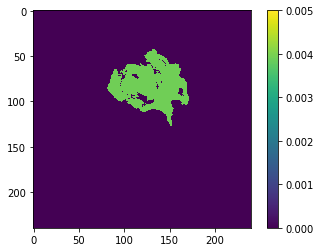
\includegraphics[width=.9\textwidth]{chapters/04_segmentation/images/evaluate1.png}
        \caption{Ground truth segment from dataset}
    \end{subfigure}%
    \begin{subfigure}[t]{.5\textwidth}
        \centering
        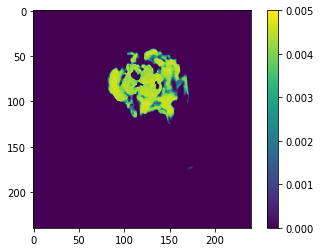
\includegraphics[width=.9\textwidth]{chapters/04_segmentation/images/evaluate2.png}
        \caption{Output from trained neural network (floating point values, not binarized)}
    \end{subfigure}
    \caption{Comparing the neural network output with the dataset ground truth shows a high correlation.}
\end{figure}


\begin{figure}[H]
\centering
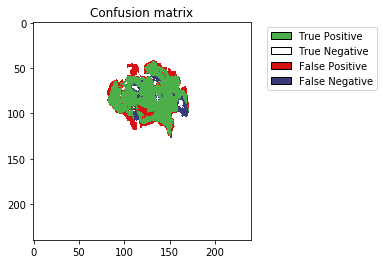
\includegraphics[width=10cm]{chapters/04_segmentation/images/confusion_matrix.png}
\caption{Confusion matrix visualization comparing the binarized network output with the ground truth segment. This confirms the high correlation between output and ground truth}
\end{figure}
